\documentclass[11pt]{article}

\usepackage[margin=1in]{geometry}
\usepackage{amsmath,amssymb,amsfonts}
\usepackage{booktabs}
\usepackage{graphicx}
\usepackage{microtype}
\usepackage[numbers,sort&compress]{natbib}
\usepackage[colorlinks=true,allcolors=blue]{hyperref}

\title{Prediction is Not Formula Fidelity:\\
Diagnosing Structure-Retention Failures in KAN Explanations}

\author{Anonymous Author(s)}
\date{\today}

\newcommand{\corefn}{f_{\mathrm{core}}}
\newcommand{\x}{\mathbf{x}}
\newcommand{\R}{\mathbb{R}}

\begin{document}
\maketitle

\begin{abstract}
Kolmogorov-Arnold Networks (KANs) are often presented as formula-friendly models for scientific discovery, but predictive accuracy alone does not establish that a learned model has recovered the correct formula structure. We study this gap using synthetic regression problems with known active variables and known interaction structure. In high-dimensional sparse interaction tasks with many nuisance variables, KANs can achieve low test error while failing to recover the formula-critical interaction. We introduce a formula-fidelity ladder that separates prediction fidelity, variable recovery, interaction-endpoint retention, and pairwise interaction recovery. Across a controlled sweep of sample size, interaction strength, and dimension, we find an empirical recovery boundary: raw KANs recover the true interaction only after enough samples and interaction signal are available. Oracle-support experiments show that KANs can fit the correct low-dimensional formula once the relevant support is supplied, while random-support and endpoint-exclusion controls show that arbitrary dimension reduction is not sufficient. We then evaluate a KAN-native stability-selection intervention that repeatedly trains full-dimensional KANs, aggregates KAN-derived variable scores, and refits a low-dimensional KAN on the stable support. This intervention improves interaction recovery in moderate-to-strong regimes, but also reveals that stability does not remove the underlying sample-size boundary. Overall, KANs are formula-capable, but not automatically formula-faithful under nuisance dimensions.
\end{abstract}

\section{Introduction}

KANs have attracted attention as neural models whose learned structure may be more interpretable and formula-like than conventional multilayer perceptrons (MLPs) \citep{liu2024kan,liu2024kan2}. This promise is especially appealing in scientific settings, where the goal is often not only to predict accurately but also to recover meaningful variables, interactions, or analytic structure. However, a low prediction error does not by itself certify that a learned model has recovered the correct formula. A model can fit the response surface well enough for prediction while relying on an incorrect decomposition, missing a weak interaction, or assigning explanatory mass to nuisance variables.

We study this gap through the lens of \emph{formula fidelity}: whether a learned explanation recovers the variables and dependency structure that define the ground-truth formula. Our central claim is deliberately modest. We do not argue that KANs cannot learn sparse interactions, nor that their failures are unique among neural models. Instead, we show that KAN explanations exhibit a \emph{structure-retention bottleneck} under nuisance dimensions. Once the correct low-dimensional support is available, KANs can fit the target formula accurately. In the full high-dimensional input space, however, recovering the formula-critical support and interaction can require crossing a recovery boundary governed by sample size, interaction strength, and support discovery.

The key diagnostic device in this paper is a formula-fidelity ladder:
\[
\text{prediction}
\;\rightarrow\;
\text{active variables}
\;\rightarrow\;
\text{interaction endpoints}
\;\rightarrow\;
\text{interaction pair}.
\]
This ladder is important because these levels can fail independently. A model may predict accurately while missing the active variables; it may recover some active variables while omitting an interaction endpoint; and it may retain both endpoints while ranking the wrong pair as the dominant interaction. Reporting only test error or only variable-level F1 therefore hides important formula-level failures.

Our contributions are:
\begin{enumerate}
    \item We define a formula-fidelity diagnostic that separates prediction error, variable recovery, endpoint retention, and pairwise interaction recovery.
    \item We introduce a controlled sparse-interaction benchmark with known active variables and known interaction structure.
    \item We show an empirical recovery boundary over sample size, interaction strength, and dimension.
    \item We use raw, RF-screened, oracle-support, random-support, and endpoint-exclusion variants to separate low-dimensional representability from full-space support discovery.
    \item We introduce a KAN-native variable-stability intervention that improves interaction recovery in moderate-to-strong regimes without relying on an external tree model as the main method.
    \item We compare against early-stopped MLP baselines, showing that the support-retention bottleneck is not unique to KAN while KAN remains strong at low-dimensional formula fitting once the support is available.
\end{enumerate}

\section{Problem Setup}

\subsection{Core Benchmark}

Our main benchmark family is
\begin{equation}
    \corefn(\x)
    =
    \sin(2\pi x_0)
    +
    x_1^2
    +
    c x_2 x_3,
    \label{eq:core}
\end{equation}
embedded in $d$ dimensions. The active variables are $\{x_0,x_1,x_2,x_3\}$, and the unique ground-truth interaction is $(x_2,x_3)$. The remaining $d-4$ variables are nuisance dimensions. Unless otherwise stated, inputs are sampled independently and uniformly, and targets are standardized using training-set statistics.

We sweep
\[
d \in \{50,100\},
\quad
n \in \{128,256,512,1024\},
\quad
c \in \{0.10,0.25,0.50,1.00\}.
\]
The main figures focus on $d=100$, while $d=50$ is reserved for appendix analysis.

\subsection{Diagnostic Variants}

We evaluate five KAN variants.
\begin{description}
    \item[Raw KAN.] The model is trained on all $d$ input variables. This tests full-space formula discovery.
    \item[RF-screened KAN.] A random forest ranks variables, and KAN is trained on the selected support. This is a diagnostic external-support intervention, not the main proposed formula-faithful algorithm.
    \item[Oracle-support KAN.] The true active variables are forced into the selected support. This separates low-dimensional representability from full-space discovery.
    \item[Random-support KAN.] A support of the same size is selected randomly. This tests whether arbitrary dimension reduction is sufficient.
    \item[Exclude-interaction KAN.] The true interaction endpoints are deliberately excluded. This tests whether the endpoints are necessary for formula recovery.
\end{description}

\subsection{KAN-Native Support Stabilization}

The RF-screened model is useful as an external diagnostic, but it is methodologically unsatisfying as a KAN explanation method: a tree model supplies the support for a spline-based neural model. We therefore evaluate a KAN-native stabilization procedure, denoted SS-KAN-V. For each target setting, we train full-dimensional raw KANs across multiple seeds or resamples and extract KAN-derived variable scores. Let $\widehat{S}^{(r)}$ be the top-$m$ variables selected by the $r$th full-dimensional KAN run. The stability frequency of variable $j$ is
\begin{equation}
    \widehat{\pi}_j
    =
    \frac{1}{R}\sum_{r=1}^{R}
    \mathbf{1}\{j\in \widehat{S}^{(r)}\}.
\end{equation}
SS-KAN-V selects the $m$ variables with the largest $\widehat{\pi}_j$, breaking ties by mean normalized KAN attribution score, and refits a low-dimensional KAN on that stable support. In the quick experiments below, $m=4$, $R\leq 10$, and the current evaluation seed is excluded from its own stability pool.

We also tested a pair-first variant that constructs support from stable pair frequencies. This variant is kept as an ablation rather than the main method: in finite samples it can prioritize stable but spurious pairs involving strong main-effect variables, thereby retaining only one endpoint of the true interaction. This failure mode is informative because it shows that pair stability should be used as a diagnostic candidate set, not as a naive support constructor.

\section{Formula-Fidelity Metrics}

Prediction fidelity is measured by test mean-squared error. Variable fidelity is measured by top-$k$ F1, where $k$ is the number of true active variables. Endpoint retention is the recall of the true interaction endpoints in the selected explanation variables. For the core benchmark, this is recall over $\{x_2,x_3\}$. Interaction fidelity is top-$k$ pair F1, where $k$ is the number of true interaction pairs. We also report the score margin
\begin{equation}
    \Delta_{\mathrm{pair}}
    =
    s(x_2,x_3)
    -
    \max_{(i,j)\neq(2,3)} s(i,j),
    \label{eq:margin}
\end{equation}
where $s(i,j)$ is the learned pair-interaction score. A positive margin means the true pair outranks every false pair.

In the main hard-regime experiments, variable scores are gradient attributions and pair scores are finite-difference mixed-interaction scores. Additional metric checks using Hessian and permutation-based interaction diagnostics are treated as robustness analyses.

\section{Results}

\subsection{Prediction is Not Formula Fidelity}

Figure~\ref{fig:prediction-vs-formula} compares raw KAN test error and interaction recovery over the hard-regime grid. The key failure mode is visible in the weak-interaction regime. For $d=100$, $c=0.10$, and $n=1024$, raw KAN reaches low test MSE around $2.5\times 10^{-3}$, but interaction F1 remains $0.0$. Prediction therefore improves before formula recovery. In scientific use cases, this distinction matters: a predictor can be useful while its recovered formula structure is wrong.

\begin{figure}[t]
    \centering
    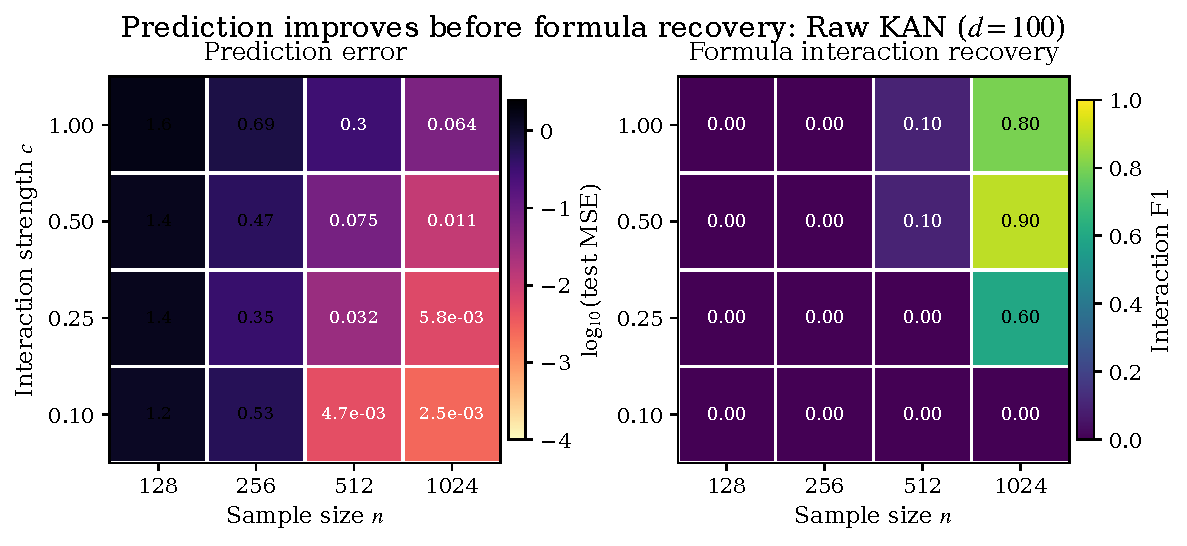
\includegraphics[width=0.92\linewidth]{../results/hard_regime/paper_figures/fig2_prediction_vs_formula_raw_d100.pdf}
    \caption{\textbf{Prediction is not formula fidelity.} For raw KAN at $d=100$, prediction error can become small even when the true interaction is not recovered. The weak-interaction setting $c=0.10$ is the clearest example: test MSE improves with sample size, but interaction F1 remains zero.}
    \label{fig:prediction-vs-formula}
\end{figure}

\subsection{A Formula-Fidelity Recovery Boundary}

Figure~\ref{fig:recovery-boundary} shows the main recovery-boundary result. We use ``recovery boundary'' rather than claiming a formal sharp phase transition: the empirical pattern is threshold-like for strong and moderate interactions, but we do not prove a discontinuous transition. For raw KAN at $d=100$, interaction recovery is near zero for small sample sizes and improves only when both sample size and interaction strength are large enough. At $n=1024$, raw KAN reaches interaction F1 of approximately $0.80$ for $c=1.00$, $0.90$ for $c=0.50$, $0.60$ for $c=0.25$, and $0.0$ for $c=0.10$.

Oracle-support KAN clarifies the mechanism. When the true support is supplied, strong and moderate interactions become recoverable, showing that KAN is not simply unable to represent the formula. However, the weakest interaction remains difficult even with oracle support, suggesting a separate detectability limit for very weak formula-critical terms. RF-screened KAN helps only when it retains the true endpoints, reinforcing that prediction-oriented support selection is not itself formula-faithful.

\begin{figure}[t]
    \centering
    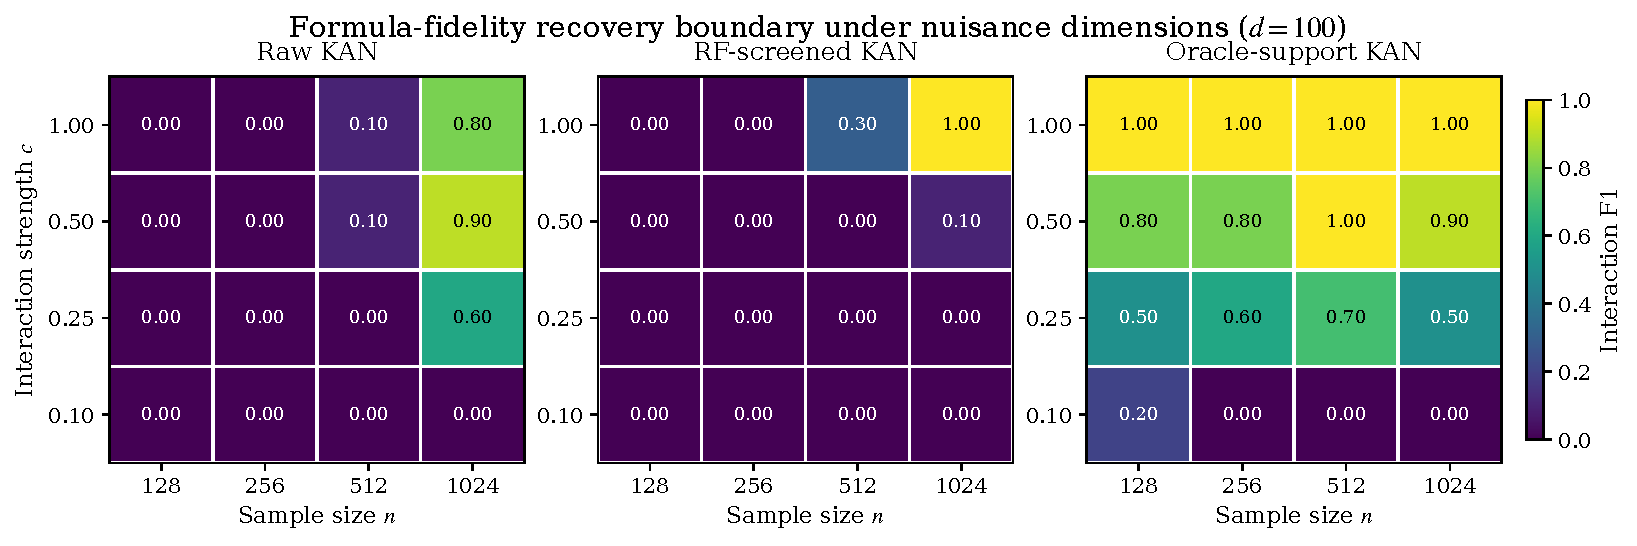
\includegraphics[width=0.98\linewidth]{../results/hard_regime/paper_figures/fig1_formula_phase_d100.pdf}
    \caption{\textbf{Formula-fidelity recovery boundary.} Interaction F1 over sample size $n$ and interaction strength $c$ for $d=100$. Raw KAN recovers the true pair only in sufficiently strong, sufficiently sampled regimes. Oracle-support KAN separates low-dimensional representability from full-space discovery. RF-screened KAN succeeds only when the screening step preserves formula-relevant endpoints.}
    \label{fig:recovery-boundary}
\end{figure}

\subsection{KAN-Native Stabilization Improves Moderate-Regime Recovery}

Figure~\ref{fig:ss-kan-boundary} evaluates SS-KAN-V on the same $d=100$ interaction family for $n\in\{256,512,1024\}$. The method is not a universal fix, but it changes the recovery boundary in the regime where the full-dimensional KAN contains enough repeated evidence for the active support. The clearest case is $c=0.50,n=512$: raw KAN has interaction F1 $0.0$, while SS-KAN-V reaches interaction F1 $1.0$ with oracle-level prediction error. For $c=1.00,n=512$, SS-KAN-V improves interaction F1 from $0.2$ to $0.6$, but still fails in seeds where the stable support misses an interaction endpoint. At $n=1024,c=1.00$, SS-KAN-V reaches interaction F1 $1.0$, compared with $0.8$ for raw KAN.

The lower-sample regime remains hard. At $n=256$, SS-KAN-V does not recover the true interaction even for $c=1.00$. For the weakest interaction, $c=0.10$, neither raw KAN nor SS-KAN-V recovers the pair across the tested sample sizes. A targeted support-capacity check at $n=512,c=1.00$ improves SS-KAN-V from interaction F1 $0.6$ with $m=4$ to $1.0$ with $m=6$, with test MSE $6.65\times 10^{-4}$, suggesting that some residual failures are near-miss support-budget failures rather than irrecoverable refit failures. Thus, stability selection is best viewed as a KAN-native support-stabilization intervention that improves moderate-to-strong regimes, not as evidence that formula recovery is solved once prediction error is low.

\begin{figure}[t]
    \centering
    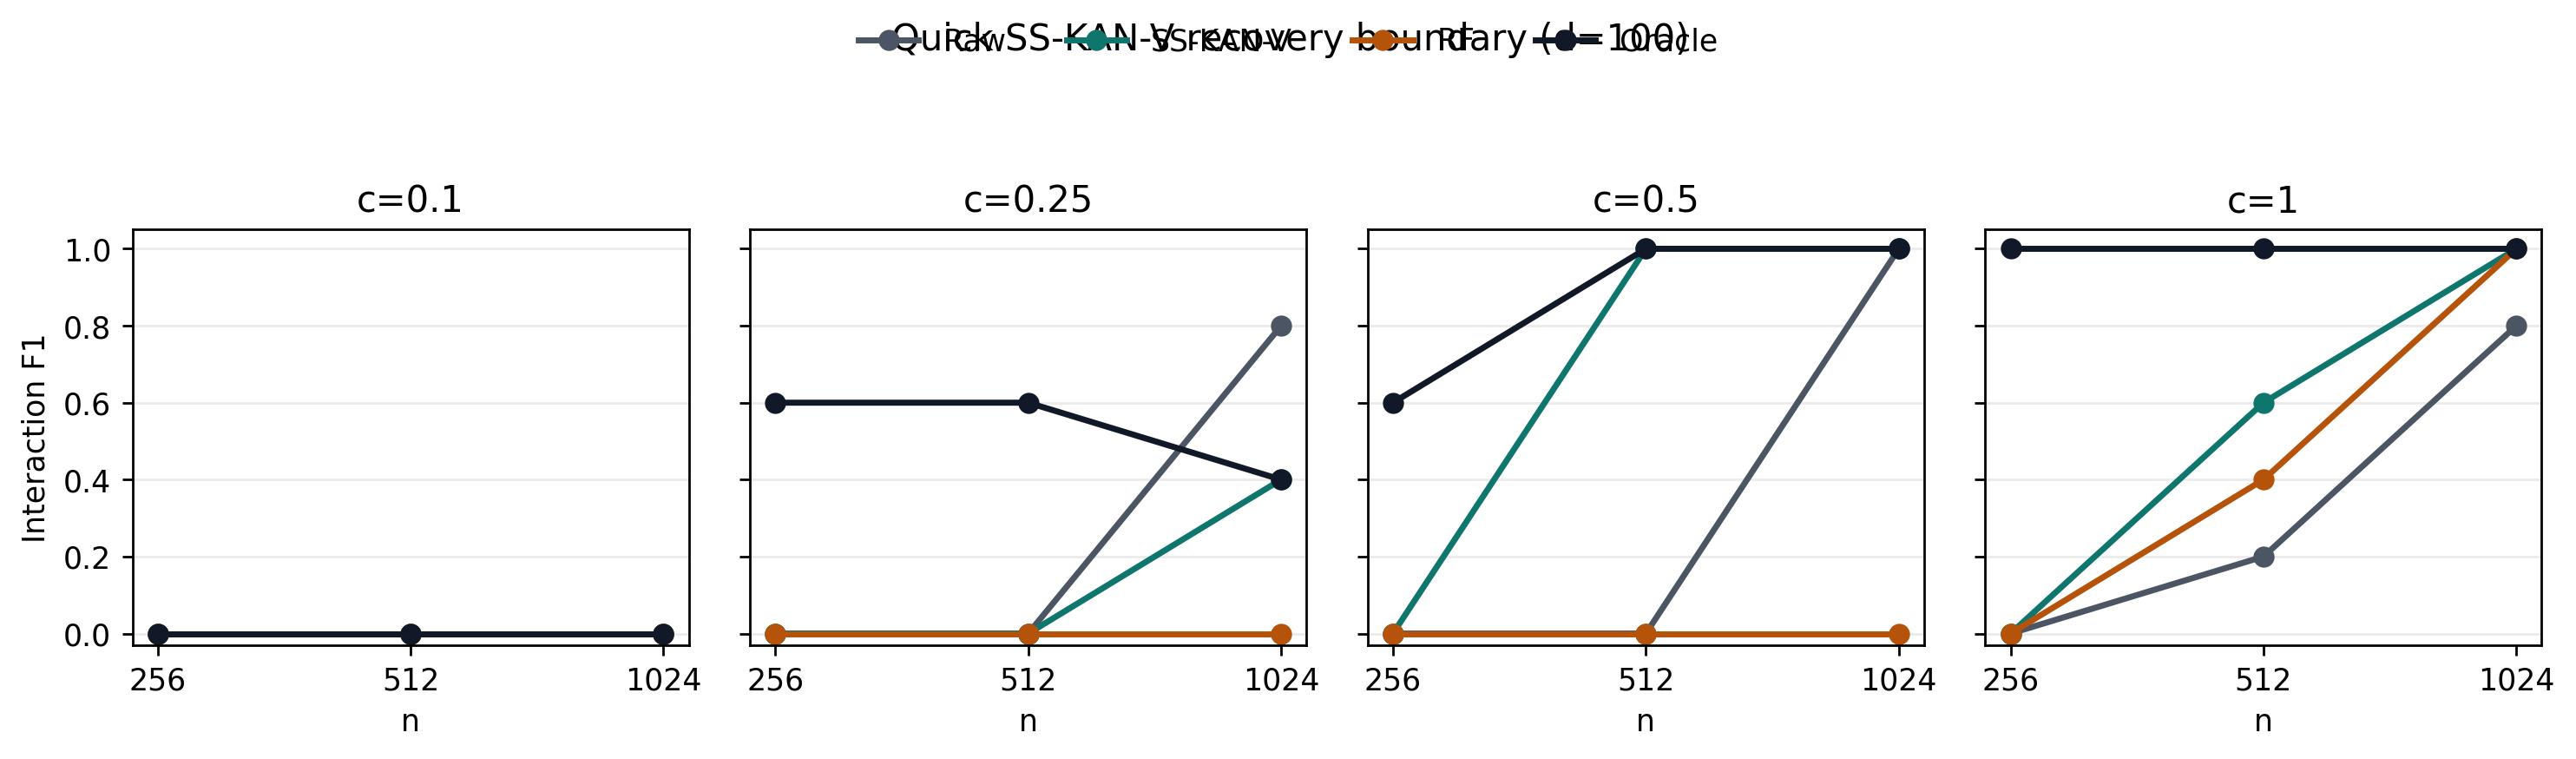
\includegraphics[width=0.98\linewidth]{../results/stability_kan/figures/quick_variable_boundary_interaction_f1.png}
    \caption{\textbf{KAN-native stability selection.} SS-KAN-V aggregates KAN-derived variable stability across full-dimensional runs, refits on the stable support, and improves interaction recovery in moderate-to-strong regimes. The strongest positive case is $c=0.50,n=512$, where raw KAN fails but SS-KAN-V recovers the interaction. The $n=256$ results show that stabilization does not remove the sample-size boundary.}
    \label{fig:ss-kan-boundary}
\end{figure}

\subsection{Variable Recovery is Not Enough}

The formula-fidelity ladder exposes failures that variable F1 alone would obscure. Figure~\ref{fig:ladder} shows variable recovery, endpoint retention, and interaction recovery for raw KAN. For $d=100$, $c=1.00$, and $n=1024$, raw KAN achieves variable F1 around $0.925$, endpoint recall around $0.85$, and interaction F1 around $0.80$. The failed seeds in this setting are diagnosed as variable-ranking failures that omit at least one true interaction endpoint. Thus, even when the variable score is high, formula recovery can still fail because the endpoints or the pair structure are not correctly retained.

\begin{figure}[t]
    \centering
    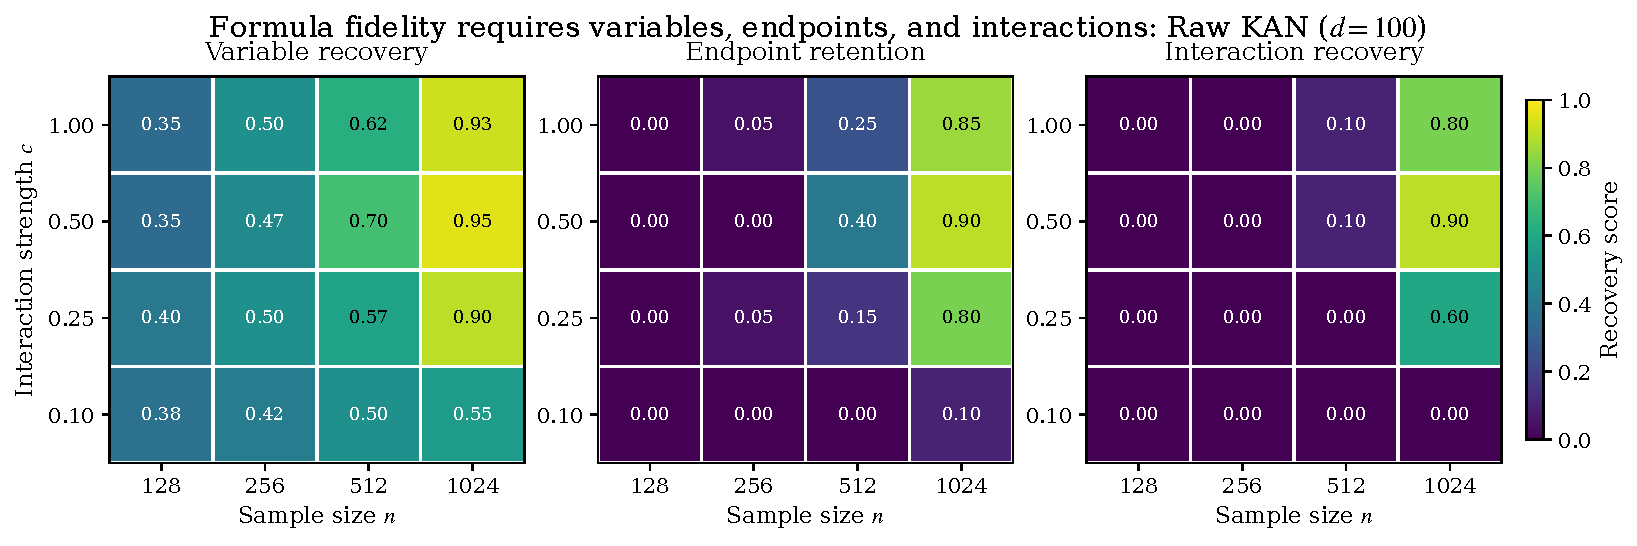
\includegraphics[width=0.98\linewidth]{../results/hard_regime/paper_figures/fig3_variable_vs_interaction_raw_d100.pdf}
    \caption{\textbf{The formula-fidelity ladder.} Variable recovery, endpoint retention, and interaction recovery are distinct diagnostic levels. High variable F1 does not guarantee that the true interaction endpoints or the true pair are recovered.}
    \label{fig:ladder}
\end{figure}

\subsection{Negative Controls}

Figure~\ref{fig:controls} shows that random support and endpoint exclusion do not recover the interaction. This rules out the simple explanation that any low-dimensional KAN is sufficient. The selected support must contain the formula-critical variables, and in particular the true interaction endpoints.

\begin{figure}[t]
    \centering
    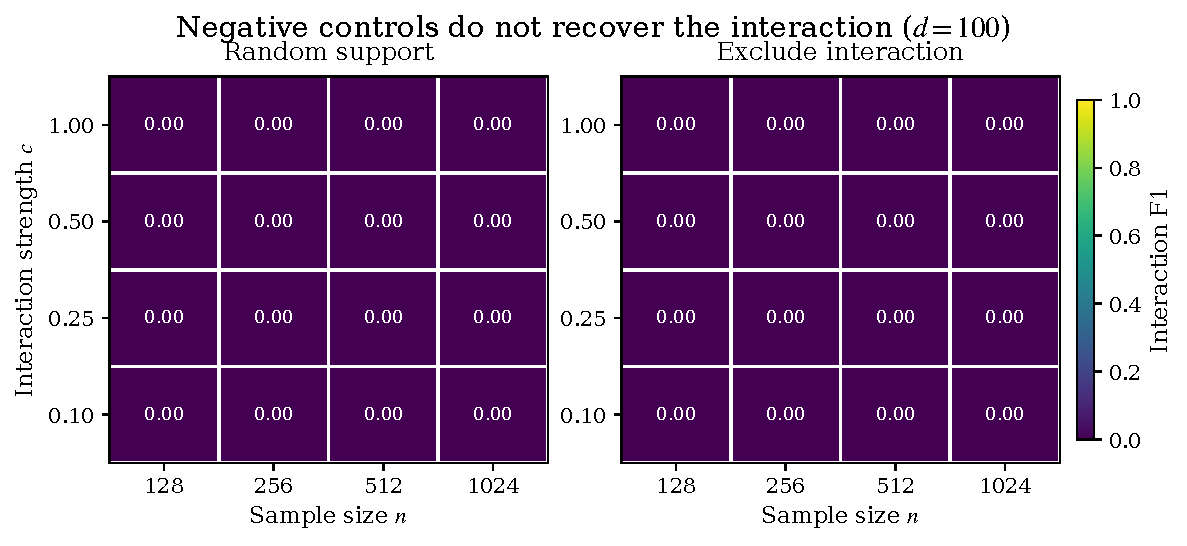
\includegraphics[width=0.82\linewidth]{../results/hard_regime/paper_figures/fig4_negative_controls_d100.pdf}
    \caption{\textbf{Negative controls.} Random-support and endpoint-exclusion controls remain near zero interaction F1, confirming that arbitrary dimension reduction is not sufficient.}
    \label{fig:controls}
\end{figure}

\subsection{MLP Baseline}

Table~\ref{tab:baseline} compares KAN and early-stopped MLP baselines in the core $d=100$, $n=1024$ setting. The MLP results show that support retention is a broad bottleneck rather than a KAN-specific pathology: once RF or oracle support is supplied, MLPs can recover the interaction ranking. However, screened and oracle-support KANs achieve much lower test MSE in the same low-dimensional support regimes, consistent with the view that KAN remains useful for formula fitting and downstream symbolic inspection once the relevant support has been retained.

\begin{table}[t]
\centering
\caption{\textbf{Core baseline comparison.} Results for the core $d=100$, $n=1024$ setting. KAN rows use $c=1.00$ from the hard-regime sweep. MLP rows use the early-stopped MLP baseline on the standard core interaction. RF and oracle support recover the interaction for both model families, but screened/oracle KAN fits the low-dimensional formula much more accurately.}
\label{tab:baseline}
\begin{tabular}{llrrrr}
\toprule
Model & Mode & Test MSE & Var. F1 & Endpoint recall & Int. F1 \\
\midrule
KAN & raw & 0.0637 & 0.925 & 0.85 & 0.800 \\
KAN & RF & 0.000334 & 1.000 & 1.00 & 1.000 \\
KAN & oracle & 0.000288 & 1.000 & 1.00 & 1.000 \\
KAN & random & 1.527 & 0.050 & 0.00 & 0.000 \\
KAN & exclude & 1.608 & 0.050 & 0.00 & 0.000 \\
\midrule
MLP & raw & 1.045 & 0.250 & 1.00 & 0.333 \\
MLP & RF & 0.832 & 1.000 & 1.00 & 1.000 \\
MLP & oracle & 0.877 & 1.000 & 1.00 & 1.000 \\
MLP & random & 1.036 & 0.167 & 0.50 & 0.000 \\
MLP & exclude & 1.035 & 0.000 & 0.00 & 0.000 \\
\bottomrule
\end{tabular}
\end{table}

\section{Mechanistic Intuition}

A pure centered interaction can be invisible to first-order marginal evidence. If $x_2$ and $x_3$ are independent and $x_3$ is centered, then for any integrable function $g$ of $x_2$ alone,
\begin{equation}
    \mathbb{E}\left[x_2 x_3 g(x_2)\right]
    =
    \mathbb{E}\left[x_2 g(x_2)\right]\mathbb{E}[x_3]
    =
    0.
\end{equation}
This does not prove a KAN-specific sample-complexity theorem. It does, however, explain why main-effect style evidence can miss a formula-critical pure interaction and why support discovery must use joint information. Any stronger local-spline signal-to-noise argument should be presented only as a heuristic appendix calculation under explicit simplifying assumptions.

\section{Limitations}

The strongest evidence in this paper is synthetic, because ground-truth formula structure is known. The theory is mechanistic rather than a formal sample-complexity result. RF screening is an external diagnostic support intervention, not a final formula-faithful method. SS-KAN-V is KAN-native, but the current evidence is a focused quick study rather than a full benchmark suite, and it improves only moderate-to-strong regimes. Interaction metrics measure pairwise dependence in the learned function; they do not by themselves prove symbolic simplification. Finally, Feynman-style formulas and additional interaction metrics are useful external checks, but the core mechanism evidence comes from the controlled sparse-interaction family.

\section{Conclusion}

KANs are formula-capable, but not automatically formula-faithful under nuisance dimensions. In high-dimensional sparse-interaction settings, prediction error can improve before the correct formula structure is recovered. The central bottleneck is not simply expressivity: oracle-support KANs can fit the low-dimensional formula, while random and endpoint-exclusion controls fail. Instead, formula fidelity depends on retaining the relevant support and interaction endpoints and then ranking the correct pair above false alternatives. SS-KAN-V shows that KAN-native stability selection can improve this bottleneck in moderate-to-strong regimes, but it also confirms that support stabilization remains governed by signal strength and sample size. These findings motivate formula-aware support stabilization and evaluation protocols that separate prediction, variable recovery, endpoint retention, and interaction recovery.

\appendix

\section{Additional Dimension Results}

The main text focuses on $d=100$. The same scripts also generate $d=50$ figures. These should be included here if space permits. The intended appendix figures are:
\begin{itemize}
    \item \texttt{../results/hard\_regime/paper\_figures/fig1\_formula\_phase\_d50.pdf}
    \item \texttt{../results/hard\_regime/paper\_figures/fig2\_prediction\_vs\_formula\_raw\_d50.pdf}
    \item \texttt{../results/hard\_regime/paper\_figures/fig3\_variable\_vs\_interaction\_raw\_d50.pdf}
    \item \texttt{../results/hard\_regime/paper\_figures/fig4\_negative\_controls\_d50.pdf}
\end{itemize}
The expected message is that reducing the number of nuisance dimensions shifts the recovery boundary but does not remove the distinction between prediction, variable recovery, endpoint retention, and interaction recovery.

\section{Metric Robustness}

The main text uses finite-difference mixed-interaction scores. Additional experiments compare Hessian scores, pair-permutation synergy, and path-based diagnostics. This appendix should report only the robust qualitative conclusion: the interaction failure is not solely an artifact of one Hessian-style metric. Path-based diagnostics should be described as qualitative because they were less stable in pilot runs.

\section{Feynman-Style External Validation}

Feynman-style formulas embedded in nuisance dimensions can be used as external validation. These results should not be the main mechanism evidence, because the core interaction family provides cleaner ground truth and cleaner controls. The appendix should report whether raw, RF-screened, and oracle-support KANs show the same support-retention pattern on formulas such as Coulomb, gravity, energy, and damped-wave variants.

\section{Heuristic SNR Intuition}

This appendix may include a heuristic signal-to-noise discussion for pure-interaction discovery under local basis parameterizations. It should not be stated as a theorem unless all independence and variance assumptions are made explicit and proved. A safe structure is:
\begin{enumerate}
    \item show first-order marginal invisibility for centered pure interactions;
    \item explain why interaction discovery requires joint evidence;
    \item discuss how nuisance dimensions increase the number of false candidate supports and false interaction pairs;
    \item state clearly that this is an intuition for the empirical recovery boundary, not a formal sample-complexity bound.
\end{enumerate}

\section{Reproducibility}

The main figures are regenerated by:
{\footnotesize
\begin{verbatim}
python experiments/augment_hard_regime_metrics.py --write_details
python experiments/plot_paper_hard_regime_figures.py \
  --dims 100 \
  --out_dir results/hard_regime/paper_figures
python experiments/make_paper_baseline_table.py
python experiments/run_stability_selected_kan_quick.py \
  --samples 256 \
  --stability_methods ss_kan_variable \
  --out results/stability_kan/quick_d100_n256_variable_detail.csv \
  --summary_out results/stability_kan/quick_d100_n256_variable_summary.csv \
  --fig_out results/stability_kan/figures/quick_d100_n256_variable_interaction_f1.png
python experiments/run_stability_selected_kan_quick.py \
  --samples 512 \
  --out results/stability_kan/quick_d100_n512_detail.csv \
  --summary_out results/stability_kan/quick_d100_n512_summary.csv \
  --fig_out results/stability_kan/figures/quick_d100_n512_interaction_f1.png
python experiments/run_stability_selected_kan_quick.py \
  --samples 1024 \
  --out results/stability_kan/quick_d100_n1024_detail.csv \
  --summary_out results/stability_kan/quick_d100_n1024_summary.csv \
  --fig_out results/stability_kan/figures/quick_d100_n1024_interaction_f1.png
python experiments/plot_stability_kan_boundary.py
python experiments/run_stability_selected_kan_quick.py \
  --functions core_interaction_c1 \
  --samples 512 \
  --stability_methods ss_kan_variable \
  --top_m 6 \
  --out results/stability_kan/robust_d100_n512_c1_topm6_detail.csv \
  --summary_out results/stability_kan/robust_d100_n512_c1_topm6_summary.csv \
  --fig_out results/stability_kan/figures/robust_d100_n512_c1_topm6_interaction_f1.png
\end{verbatim}
}
The full hard-regime matrix can be rerun with:
{\footnotesize
\begin{verbatim}
./run_hard_regime_matrix.sh
\end{verbatim}
}
See \texttt{docs/reproducibility\_checklist.md} for the current artifact map.

\bibliographystyle{plainnat}
\bibliography{references}

\end{document}
